\chapter{Fixed Time Quantum}

Fixed Time Quantum\cite{ftq} is a tool for creating measurements of operating system noise, allowing users to do quantitative analysis 
with
standard tools such as Matlab and GNU Octave.

FTQ has found wide use in both the research and commercial world, having become one of the standard measurement tools for OS noise. 
Both IBM and Cray have used it to help tune their operating system kernels for minimal noise. 
FTQ results supported Cray's decision to move to Compute Node Linux, replacing the Catamount Light Weight Kernel originally delivered with those systems. Real 
application results supported the initial results from FTQ. 

The distinguishing feature of FTQ is that it measures work per fixed amount of time, rather than the more traditional time taken to do a fixed amount of work. The distinction is subtle but essential.  FTQ is written to carefully ensure that the time samples are for a fixed amount but also that the sampling interval is {\em stationary}. FTQ ensures this property by starting each sample interval at the correct point in team even if, due to interference, the previous sample interval took too long. For more discussion of how this is done the reader is referred to the original paper. 

As mentioned, FTQ allows users and vendors to use quantitative, rather than qualitative analysis.  As an example we will walk through real data taken on 
Blue Gene/P on a very early implementation of Plan 9. 
The FTQ program produces two output files: a so-called "counts" file, and a times file. These two files allow a user to reconstruct how much work was done per interval. The files 
are useful independent of each other: the counts data gives some idea of how much work was done, so
that the same binary, under different operating system, can compare how well the applications run.
The times data can be used to determine how well the algorithm that maintains stationary sampling is
doing its job; deviations of the time from a desired baseline can point to operating system, virtual
machine,  or even hardware problems: the times file was used to diagnose virtual machine interference on the Purple system at LLNL. Combined, the two files can be used for deeper analysis, combining both work and time information. 

While the raw data is useful, it is possible to misread too much into a raw data plot. In the original paper we showed two traces, one of them generated by white noise and the other by a very well-defined signal. To the naked eye, they are indistinguishable. Further processing of the data is essential to ensure that the measured data represents information, not white noise. 

In Figure \ref{rawdata}, we show a similar plot for three FTQ runs, on CNK, Linux, and Plan 9. What is of interest are not the actual numbers -- the Plan~9 binary 
is a different binary -- but the occurrence of spikes in the graph. One can gain some information immediately: there is clearly periodic interference of the same 
frequency for each operating system. Further investigation revealed that the 64-bit processor clock, comprised of two 32-bit counters, had a glitch when the
low-order 32-bit counter rolled over, leading to a slightly longer sample interval at that point. The algorithm quickly resynchronized, however, such that the 
counts over a long period were correct. This spike can easily be misinterpreted in the time domain graph; it does not have any impact on the frequency domain graph. 
\begin{figure}[h]
\begin{center}
 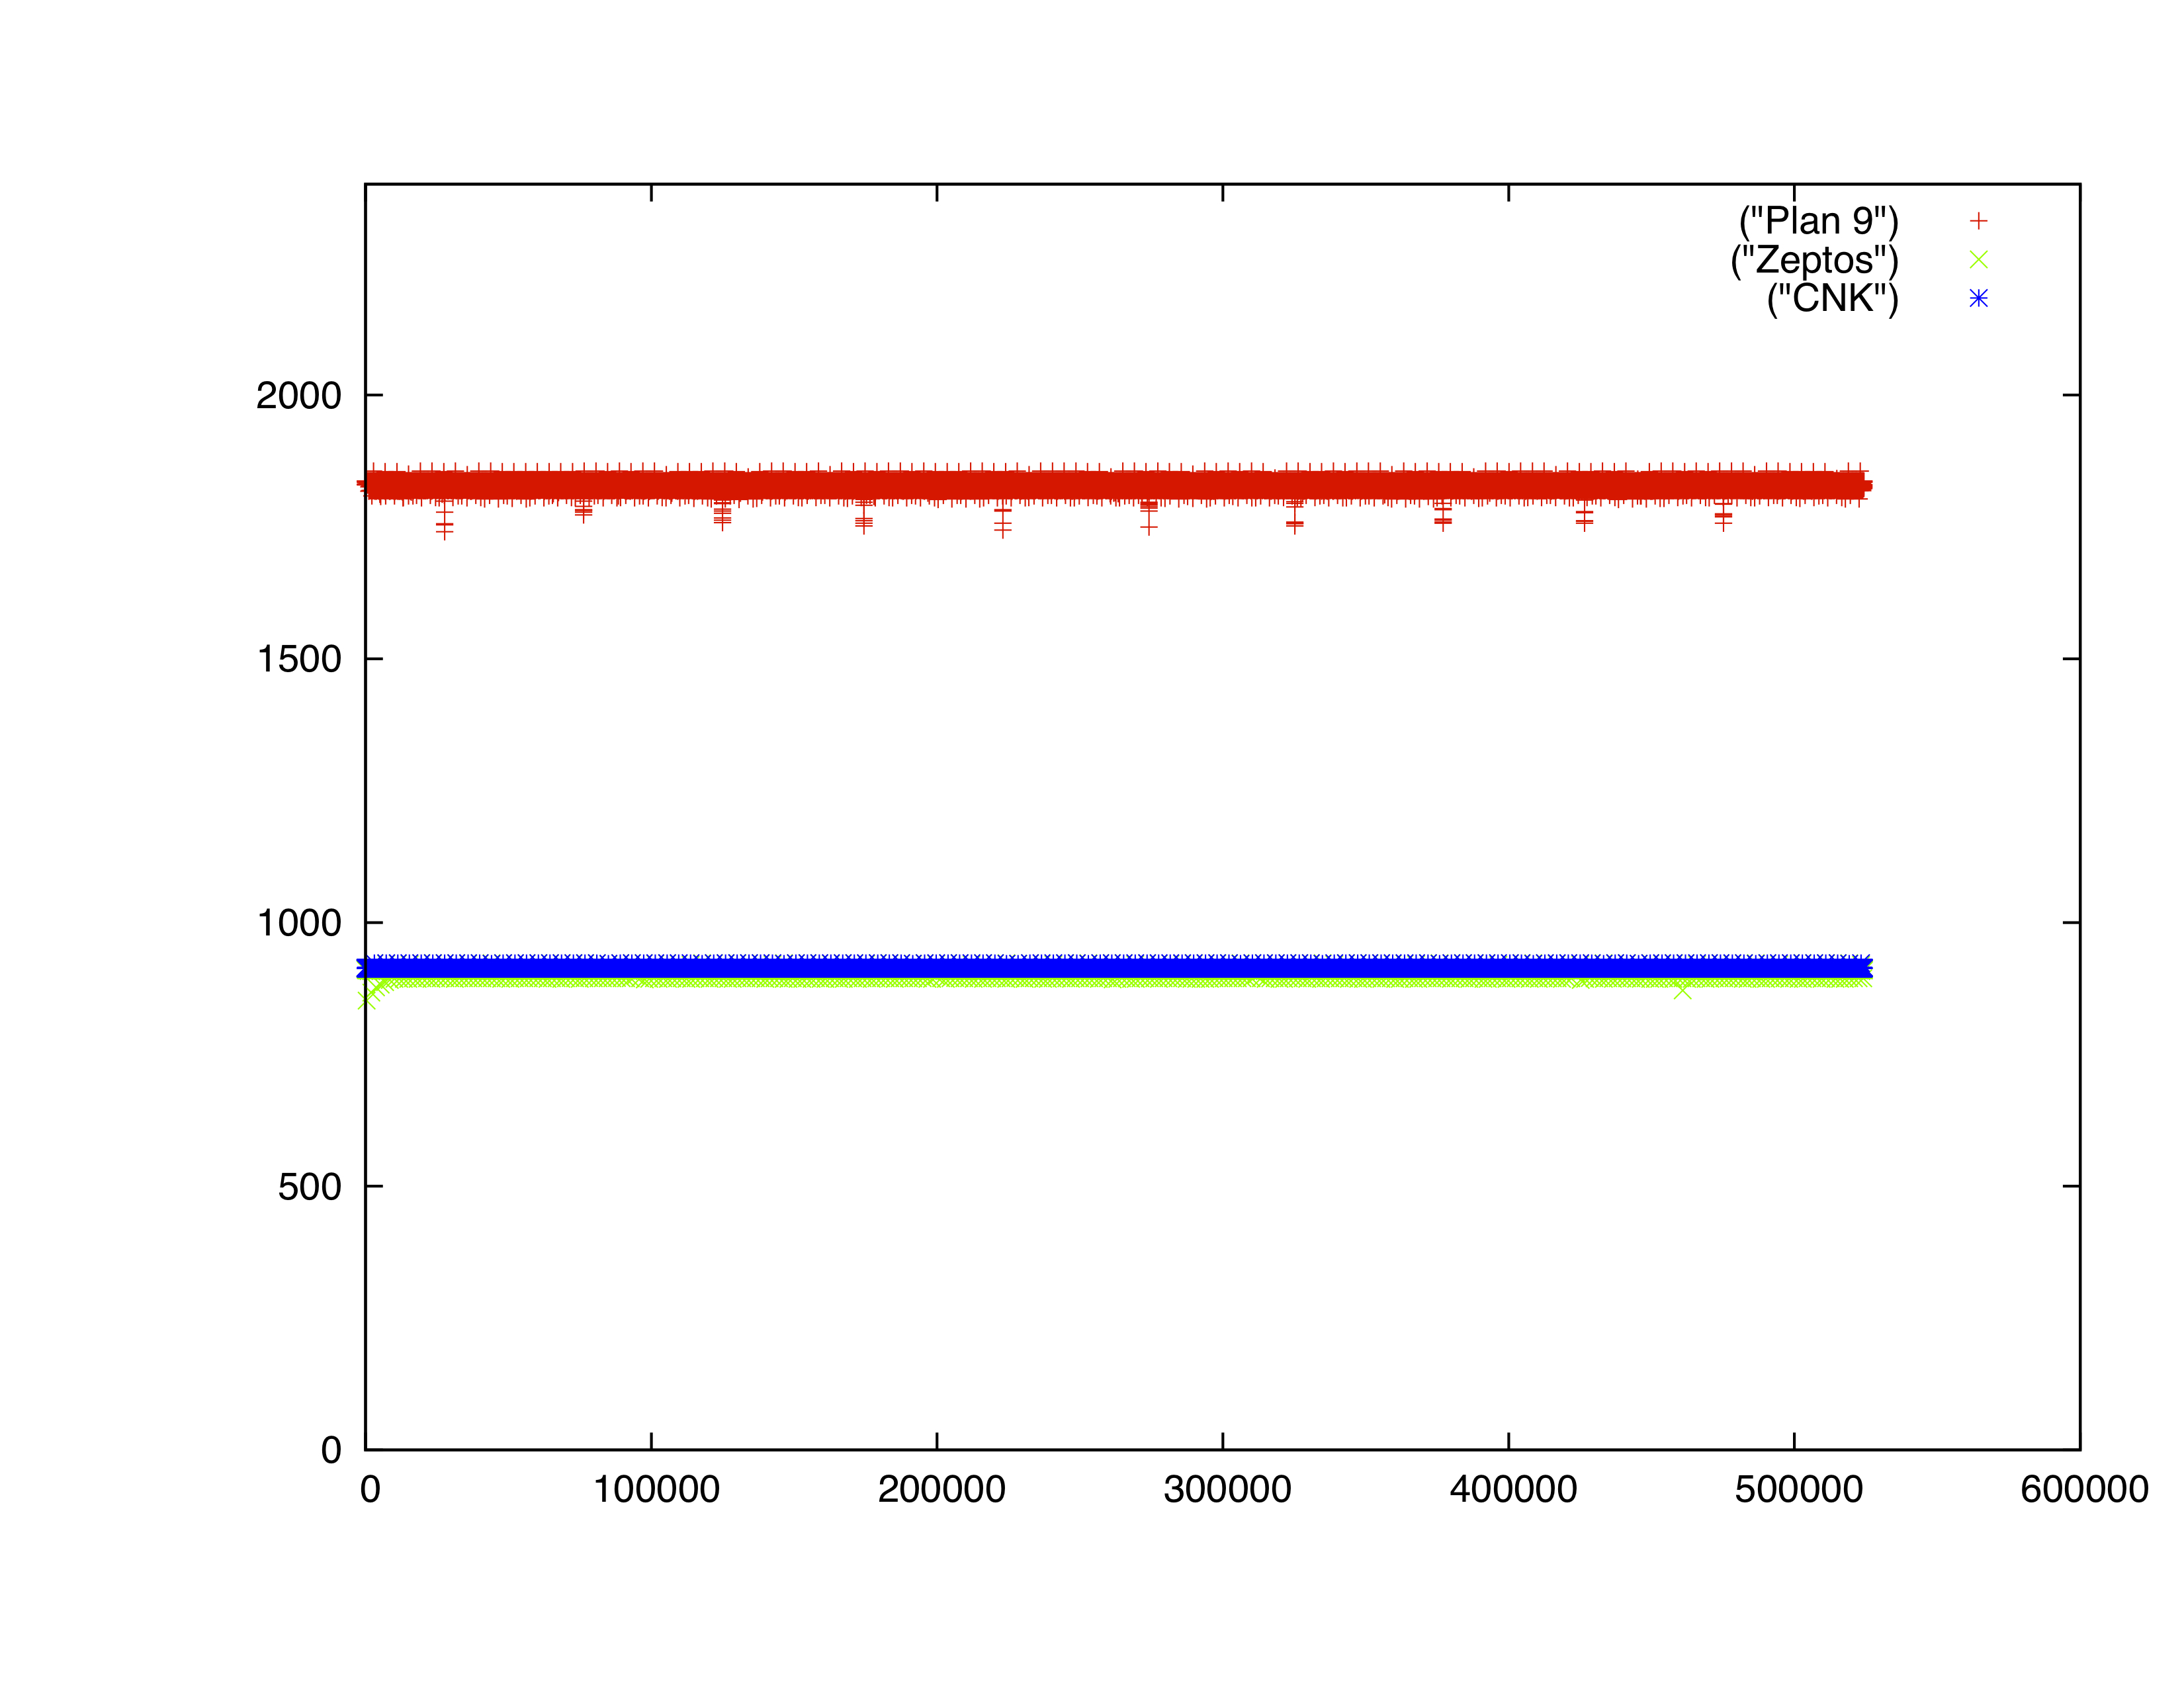
\includegraphics[width=4in]{raw.jpg}
 \caption{{\bf A plot of FTQ 'count' data for three Blue Gene/P operating systems, with sample
 number on the X axis and unit-less work on the Y axis.}}
\label{rawdata}
\end{center}
\end{figure}

Converting this data to the fequency domain is relatively straightforward. We present the octave script in Figure \ref{octave}. 
\begin{figure}[h]
\begin{center}
\begin{verbatim}
samples = readcounts('9ftq63_0_counts.dat');
samples = fitmax(samples);
[Psd,w] = pwelch(samples,[],[],[],810);
\end{verbatim}
\caption{Octave script for processing raw FTQ data. We only use the counts file in this case.}
\label{octave}
\end{center}
\end{figure}
The program reads the file in using a function that returns a one-dimensional vector. The function
{\tt fitmax} normalizes all the values in the vector to the maximum value. Finally, 
the code calls the octave pwelch function, which generates two vectors: a power spectrum estimation (Psd) and a set of frequencies(w). The parameters are the samples, and the 
cycle counter 
frequency (810 Mhz.). 
We show a plot of the Power spectral density for the three operating systems in Figure \ref{psd}
\begin{figure}[htbp]
\begin{center}
 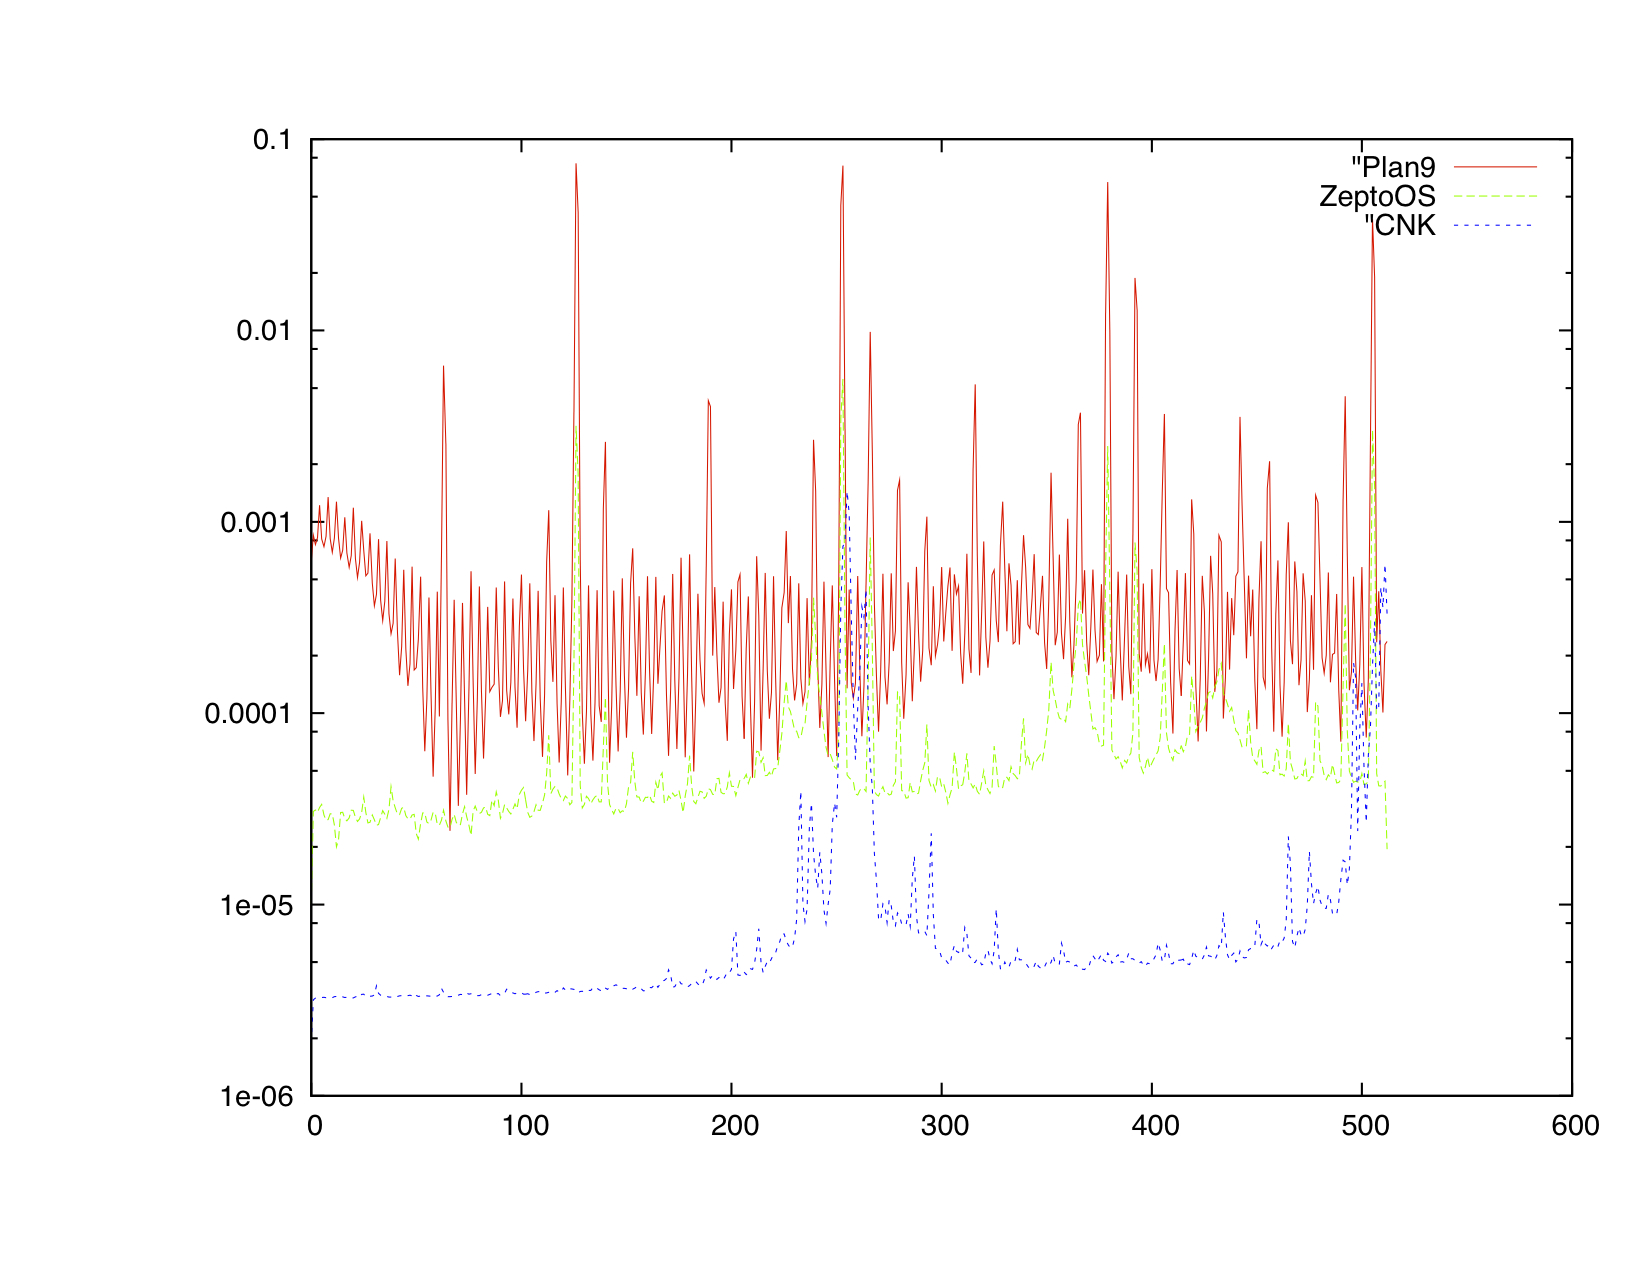
\includegraphics[width=5in]{spectrum.jpg}
\caption{{\bf Power Spectral Density for the three operating systems, Frequency in HZ on the x axis
and unit-less amplitude on the Y axis.}}
\label{psd}
\end{center}
\end{figure}

The graph shows that CNK has a better noise figure than either of its two
more general purpose competitors. It is also possible to see
the frequencies at which noise spikes occur. In fact, an earlier version 
of this chart revealed a very distinct noise spike at 30 HZ. which we 
eliminated. Finally, it is easy to see that, while there is an apparent similarity in the time
domain between CNK and ZeptoOS noise,they are not at all similar in the
frequency domain. One can not simply look at raw data graphs and 
reveal all the hidden information. 

FTQ allows us to quantitatively measure and analyze noise, using standard 
signal processing techniques. Spectral components of noise can be measured, 
traced back to their source, and eliminated. 

